\documentclass[11pt]{article}
\usepackage[a4paper,margin=1in]{geometry}
\usepackage[T1]{fontenc}
\usepackage{mathptmx}
\usepackage[scaled=0.9]{helvet}
\usepackage{courier}
\usepackage{xcolor}
\usepackage[utf8]{inputenc}
\usepackage{microtype}
\usepackage{booktabs}
\usepackage{array}
\usepackage{tabularx}
\usepackage{enumitem}
\usepackage{tikz}
\usetikzlibrary{arrows.meta,positioning,shapes.geometric,fit,patterns}
\usepackage[numbers,sort&compress]{natbib}
\usepackage[colorlinks=true,linkcolor=blue!50!black,citecolor=blue!50!black,urlcolor=blue!50!black]{hyperref}
\setlist{nosep,leftmargin=1.4em}
\definecolor{codegreen}{RGB}{0,120,0}
\definecolor{barblue}{RGB}{38,110,180}
\definecolor{barorange}{RGB}{210,125,30}
\definecolor{bargray}{RGB}{120,120,120}
\newcommand{\code}[1]{\textcolor{codegreen}{\texttt{#1}}}

\begin{document}
\begin{center}
{\LARGE\bfseries Agent-Causality: Declared Dependency Tracing and\\[2pt]
Counterfactual Sensitivity Analysis for Multi-Agent Systems\par}
\vspace{1.4em}
{\large\bfseries Vasant Kumar Mogia\par}
\vspace{0.3em}
{\large Psionics\par}
\vspace{0.4em}
{\large{vasant@psioniclabs.tech}\par}
\vspace{0.3em}
{\href{https://psionic-labs.github.io/Agent-Causality/}{\textcolor{blue!80!black}{https://psionic-labs.github.io/Agent-Causality}}\par}
\vspace{0.5em}
\end{center}
\vspace{1em}

\begin{abstract}
AI systems built from several cooperating agents are easy to record but hard to debug. A conventional log shows what happened in order, but not which earlier events a failure structurally depends on. The problem is harder when agents run in parallel and their outputs merge into one decision, because a failure may depend on one branch, on several, or on their joint ancestry. We present Agent-Causality, an open-source tool that records a dependency graph with explicit parent links, computes structural slices and provenance grades, and supports decision contracts with deterministic counterfactual replay. From the graph, the tool trims a run to structural ancestors, traces values to their sources with exact or coarse labels, and tests whether recorded inputs, alone or jointly, change a registered merge decision in replay. It also produces a structured summary and keeps optional model-written text in a separate block. We describe the design, assumptions, and limits; the evidence is five deterministic fixtures, a synthetic shared-state test, an offline single-port replacement test, and a five-task live pilot that did not exercise the injected failures. We do not claim actual causation. We outline proposed combinations with agent frameworks, test runners, approval systems, and security gateways.
\end{abstract}

\noindent\textbf{Keywords:} multi-agent systems, LLM agents, dependency tracing, failure attribution, observability, counterfactual sensitivity analysis, AI agent debugging, AI safety, trustworthy AI, AI agent reliability

\section{Introduction}
Modern AI applications are no longer a single model answering a single question. A planner agent may hand work to a researcher agent and a coding agent, each of which calls tools, reads and writes shared memory, and sends results back to be merged. When the final answer is wrong, the developer faces a trace of hundreds of events and must decide which recorded events the failure depends on.

Conventional observability tools are good at showing the trace; they answer ``what happened?'' This paper asks a narrower second question: which earlier events does a failure structurally depend on, and which recorded inputs change a registered decision when replayed? Agent-Causality is built around that record. It does not discover causal effects from observational traces.

\vspace{1em}  

This paper makes four contributions, each tied to a section and a repository artifact:
\begin{enumerate}
\item A capture model that records events and explicit parent links, with shared-resource versioning for registered resources (Sections~\ref{sec:idea} and~\ref{sec:capture}--\ref{sec:shared}; \code{sdk/events.py}, \code{sdk/memory.py}).
\item Structural slicing and exact/coarse provenance grades (Sections~\ref{sec:slice}--\ref{sec:provenance}; \code{core/slicing.py}, \code{core/provenance.py}).
\item Decision contracts and deterministic local replay with Shapley-style and functional-interaction summaries (Sections~\ref{sec:contracts}--\ref{sec:minimal}; \code{core/decision.py}, \code{core/replay.py}).
\item Two adapters and committed evaluation artifacts (Sections~\ref{sec:combined}--\ref{sec:eval}; \code{adapters/langgraph}, \\ \code{adapters/opencode}, \code{benchmark/results}).
\end{enumerate}
These are engineering and empirical contributions. None of them is a method for identifying causal effects from logs. 

The paper has three goals. First, to explain declared dependency tracing and counterfactual sensitivity analysis for a reader without a causal-inference background (Sections~\ref{sec:problem} and~\ref{sec:idea}). Second, to describe the system and what it supports on its own (Sections~\ref{sec:system}--\ref{sec:alone}). Third, to describe proposed combinations with other tools (Section~\ref{sec:combined}). Assumptions and threats to validity appear with the limitations (Section~\ref{sec:limits}), and related work follows in Section~\ref{sec:related}.

\section{The Problem}\label{sec:problem}
\subsection{A trace is a list, a failure is a web}
A trace is usually a numbered list of steps. A list shows order but not dependence: step 8 may have depended only on steps 4 and 7, but the list does not say so. In a multi-agent system this matters because agents work in parallel branches that later merge. Figure~\ref{fig:dag} shows the shape.

Consider a customer-approval decision that combines two reports: one agent checks whether the customer is eligible, another checks a risk score. The decision approves if the customer is eligible and the risk is low. Suppose the recorded status is wrong and the recorded risk is wrong in a way that is harmless in isolation, but together they produce a wrong approval. Neither branch alone is sufficient in this example. The graph shows that both branches are structural ancestors of the failure; whether both are functionally necessary is a separate question, tested only when a decision contract and a registered evaluator are available. A trace that shows one branch at a time cannot reveal the merge.

\subsection{Four shapes of failure}
When two branches feed one decision, a failure can take one of four conceptual shapes:
\begin{itemize}
\item \textbf{Single cause:} one input is enough to change the outcome.
\item \textbf{Either cause:} either input alone would change the outcome.
\item \textbf{Joint cause (functional interaction):} both inputs must be present together; neither alone changes the registered decision in replay.
\item \textbf{Dependent cause:} one input changes how the other should be read. The current implementation has no dedicated test for this case; it is included here for completeness.
\end{itemize}
A useful debugger should distinguish these patterns instead of attributing the failure to the last step or the loudest error.

\section{The Core Idea}\label{sec:idea}
Agent-Causality turns a run into three connected views: the \emph{execution history} (what happened, in order), the \emph{dependency graph} (which events carry links to earlier events), and \emph{provenance} (where a value came from, and how exact the link is). The building blocks are few:
\begin{itemize}
\item \textbf{Event:} one thing that happened, such as a model call, a tool call or result, a memory read or write, or an agent starting or finishing.
\item \textbf{Parent links:} each event can carry a list of earlier events whose information it used. A merge event can have several parents. The current event schema stores parent IDs only; it does not store a separate edge-type field.
\item \textbf{Append-only log:} the SDK and SQLite store append events rather than updating them. This is a code convention, not a database-enforced guarantee: the schema has no immutability trigger, so a direct database update could rewrite history.
\item \textbf{Logical clock:} each event gets a logical sequence number (a Lamport-style clock~\cite{lamport1978}). A new event receives a sequence greater than all of its parents' sequences. Acyclicity therefore follows from sequence allocation under normal capture; there is no separate cycle validator.
\item \textbf{Snapshot:} an optional saved copy of \emph{one agent's} state. Snapshots are a library feature and are not used by the default analysis path, which reconstructs from the event log instead.
\end{itemize}

\paragraph{Terminology.} We distinguish six things. A \emph{declared edge} is a parent link emitted by instrumentation or application code (for example, a tool result paired with its tool call, or a read linked to a prior write). An \emph{order-inferred edge} is synthesized from execution order by an adapter; the LangGraph adapter currently does this (Section~\ref{sec:integrations}). An \emph{exact data link} is a provenance link where a value was copied or passed directly through a tool or assignment. 

\vspace{1em}

A \emph{coarse model boundary} marks a value that passed through a language model, where the mapping from input parts to output parts is unknown. A \emph{structural ancestor} is any event reachable by walking parent links backward. \emph{Functional influence} is a change in a registered decision when a recorded input is replaced during replay, holding the other recorded values fixed. We say \emph{joint ancestry} when several branches appear in a structural slice, and \emph{functional interaction} when a registered decision changes only under their joint intervention. Neither is a claim of actual causation.

\vspace{1em}    

One design rule matters: the core SDK records only dependencies that were declared or observed (for example, a tool result paired with its tool call, or a read of a value an earlier event wrote). It does not guess dependencies from event order. One decorator path, \code{merge\_decision}, wires each port to the most recent prior tool result whose output equals the port value; this is value matching and can be ambiguous when values repeat. The lower-level contract API can specify a source event explicitly. The LangGraph adapter is a further exception: it synthesizes order-inferred edges and chains sequential siblings (Section~\ref{sec:integrations}). The event schema does not mark which edges came from which rule, so downstream consumers must know which adapter produced a graph.

\begin{figure}[t]
\centering
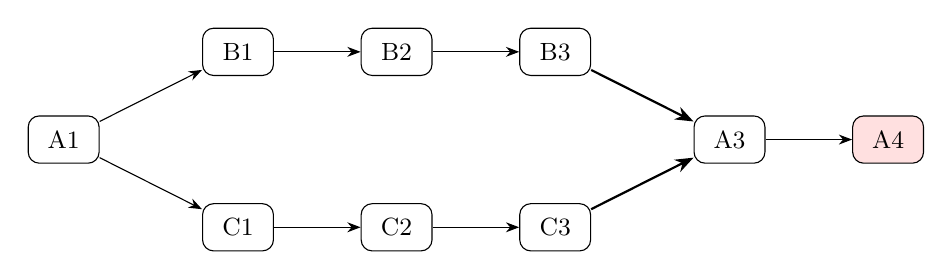
\begin{tikzpicture}[node distance=1.1cm,>=Stealth,
  ev/.style={draw,rounded corners,minimum width=0.9cm,minimum height=0.6cm,font=\small},
  fail/.style={draw,rounded corners,minimum width=0.9cm,minimum height=0.6cm,font=\small,fill=red!12}]
  \node[ev] (A1) {A1};
  \node[ev,above right=0.5cm and 1.3cm of A1] (B1) {B1};
  \node[ev,right=of B1] (B2) {B2};
  \node[ev,right=of B2] (B3) {B3};
  \node[ev,below right=0.5cm and 1.3cm of A1] (C1) {C1};
  \node[ev,right=of C1] (C2) {C2};
  \node[ev,right=of C2] (C3) {C3};
  \node[ev,below right=0.5cm and 1.3cm of B3] (A3) {A3};
  \node[fail,right=of A3] (A4) {A4};
  \draw[->] (A1)--(B1); \draw[->] (A1)--(C1);
  \draw[->] (B1)--(B2); \draw[->] (B2)--(B3);
  \draw[->] (C1)--(C2); \draw[->] (C2)--(C3);
  \draw[->,thick] (B3)--(A3); \draw[->,thick] (C3)--(A3);
  \draw[->] (A3)--(A4);
\end{tikzpicture}
\caption{A branching run. A planner (A) starts a researcher (B) and a coder (C). Their outputs merge at A3, which feeds the failing final answer A4. A3 has two parent links, so a simple list or tree cannot represent it.}
\label{fig:dag}
\end{figure}

\section{How the System Works}\label{sec:system}
The system follows a pipeline from recording to a structured summary (Figure~\ref{fig:pipe}).

\begin{figure}[t]
\centering
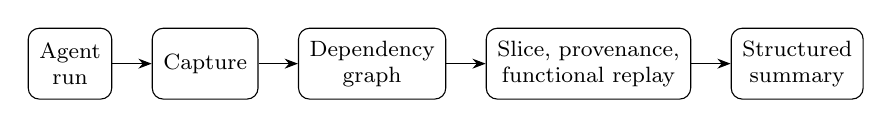
\begin{tikzpicture}[node distance=0.5cm,>=Stealth,
  s/.style={draw,rounded corners,align=center,font=\footnotesize,minimum height=0.9cm,inner sep=4pt}]
  \node[s] (a) {Agent\\run};
  \node[s,right=of a] (b) {Capture};
  \node[s,right=of b] (c) {Dependency\\graph};
  \node[s,right=of c] (d) {Slice, provenance,\\functional replay};
  \node[s,right=of d] (e) {Structured\\summary};
  \draw[->] (a)--(b); \draw[->] (b)--(c); \draw[->] (c)--(d); \draw[->] (d)--(e);
\end{tikzpicture}
\caption{Overall flow, from a running agent to a structured, evidence-linked summary.}
\label{fig:pipe}
\end{figure}

\subsection{Capture}\label{sec:capture}
A small SDK records events as agents run. In Python, a developer initialises it with a storage path and marks agent functions and merge decisions with decorators. Events go to SQLite by default. PostgreSQL is a storage-layer option; the direct \code{causality.init} path opens SQLite.

The OpenCode and LangGraph adapters redact secrets before storage and are fail-open: capture failures do not propagate into the agent. Direct SDK capture is neither fail-open nor redacted by default. Its events go through the raw append path, where an append error can propagate, and it passes no redactor. The SDK's optional \code{PayloadRedactor} is shallow (top-level keys only) and is disabled by default. The adapters use deeper key- and value-based redaction, but it is not a guarantee that every secret is removed.

\subsection{Shared state}\label{sec:shared}
Agents often talk indirectly, for example one writes a shared file or memory key and another reads it. For resources registered with the SDK, each resource carries a version number and its last writer. When an agent reads the resource, the system links that read to the write that produced the value. This applies to registered memory keys and to tool results whose adapter supplies a resource URI; arbitrary databases and files are not automatically versioned.

\subsection{State reconstruction}
To answer ``what did this agent know at this point?'', the system can reconstruct one agent's state at a logical sequence by replaying its events. A snapshot store can shorten the replay, and a stored hash can verify a rebuilt state. These are optional library features. The default \code{why} and \code{explain} paths do not pass a snapshot store, do not verify the hash, and reconstruct only one agent at a time. The paper does not claim global, cross-agent state reconstruction or snapshot-accelerated analysis.

\subsection{Structural slice}\label{sec:slice}
Given a failed event, the system walks backward through parent links and collects everything the failure is structurally connected to. This \emph{structural slice} is cheap: it follows existing links and re-runs nothing. The implementation runs in time linear in the number of events and edges. As an illustration only, a 500-event run might shrink to a dozen events; this is not a measured result. A slice shows what a failure was connected to, not proof that every included event had an effect.

\subsection{Provenance}\label{sec:provenance}
Provenance traces a value back to its origin and is open about reliability. If a value passed through a tool call or a direct copy, the link is \emph{exact}. If it passed through a language model, no one can say which part of the input produced which part of the output, so the link is marked \emph{coarse}. A coarse link is never presented as exact. An exact link is a data link, not a claim of causal influence.

\subsection{Decision contracts}\label{sec:contracts}
A merge decision is described as a small contract: a name for each input (a ``port''), where it came from, its recorded value, and a neutral baseline value to use when testing without it. A contract can mark a decision as side-effecting, but the flag defaults to false. Developers can then ask ``why did this decision go this way?'' instead of ``show the ancestors of event 42.''

\subsection{Counterfactual replay and functional interaction}\label{sec:replay}
A slice shows what was structurally connected. To test functional influence, the system asks a ``what if'' question: what would the decision have been if this one input had been normal? It freezes the recorded outputs of earlier branches and calls the registered evaluator for the decision, swapping in baseline values for chosen inputs. This is a targeted replacement of a value, not deletion of text, so the evaluator receives a well-formed input. It does not re-run the model or any earlier agent branch.

Replay calls application code. It cannot inspect the evaluator's body, so it cannot determine whether that code sends email, writes a database, or performs another external action. The current guard checks explicit contract metadata and recorded port values for side-effect indicators, but it cannot guarantee safety. Evaluators must be pure. The system does not provide a sandbox for impure evaluators.

\vspace{1em}   

Running the evaluator with each combination of inputs present or replaced shows which inputs change the outcome alone and which change it only together. The system summarises this with Shapley-style scores~\cite{shapley1953} and a pairwise functional-interaction index~\cite{grabisch1999}. The functional-interaction index measures joint sensitivity beyond separate effects under the registered evaluator; it is not evidence of causal influence between agents. Exact subset enumeration currently supports decisions with up to four input ports. For a fixed contract and code version, replay is deterministic when the evaluator is deterministic: repeated calls with identical inputs return identical outcomes. The replay harness does not itself sample a language model; for the deterministic evaluators used here, duplicate evaluations are identical copies, not stochastic trials, and we draw no model-uncertainty conclusion from them.

\subsection{Minimal slicing}\label{sec:minimal}
Where a structural slice is still too large, the system can search for a smaller subset that still satisfies a test predicate, using delta debugging~\cite{zeller2002}: repeatedly remove parts and check whether the predicate still holds. This needs replay, so it runs only on request. The result is a \emph{required-cause preservation proxy relative to that predicate}; it is not causal minimality. A different predicate can yield a different subset.

\subsection{Explanation and visual explorer}
The final step produces a short structured summary. It draws on the structural slice, contract, and replay evidence. An optional language model can phrase it, but that text is kept in a separately labelled block and is not mixed with the recorded evidence. The structural-slice output carries a systematic note that ancestry is not proof of influence. Other statements are not checked by a general claim-level evidence verifier. The offline renderer used by the bundled example also has fixture-specific branches (Section~\ref{sec:example}); it is not a general explanation capability. A Visual DAG Explorer shows the graph and a per-agent timeline, lets the user click any event to see its parents and children, and highlights the failure path.

\section{Fixture Walkthrough: Customer Approval}\label{sec:example}
This section walks through the bundled customer-approval fixture. It demonstrates the fixture path, not a general capability. The offline renderer has hardcoded branches for \code{customer\_status} and \code{risk\_score}.

The fixture captures two agent results and a wrong approval. The customer was marked eligible with a risk score of 0.2, so the decision approved; the expected values were ``ineligible'' and a risk of 0.8. The output (shortened; the fixture labels the last quantity ``interaction'') is:
\begin{quote}\small
Outcome: approved\\
Diagnosis: The terminal event is marked `failure' because the decision returned `approved' with customer\_status=`eligible' and risk\_score=0.2.\\
Evidence:\\
- Minimal tested chain: customer\_status + risk\_score -> decision -> terminal failure\\
- Recorded inputs were customer\_status=`eligible' and risk\_score=0.2; their canonical baselines are `ineligible' and 0.8.\\
- Reported functional-interaction index (printed as ``interaction''): 1.0\\
Limitations: the evidence does not establish why the upstream tools produced these values.
\end{quote}
Two things stand out. The fixture reports the combination through a functional-interaction index rather than attributing the failure to one branch, and it states what it cannot tell, namely why the upstream tools produced those values. Because the renderer is fixture-specific, this is a demonstration of the bundled path, not evidence of a generic diagnosis capability.

\section{What the Tool Supports on Its Own}\label{sec:alone}
Used alone, with the SDK, a store, and the explorer, Agent-Causality supports the capabilities in Table~\ref{tab:alone}. ``Partial'' means the mechanism exists but has a stated scope limit.

\begin{table}[h]
\centering\small
\begin{tabularx}{\linewidth}{@{}>{\raggedright\arraybackslash}p{4.8cm}>{\raggedright\arraybackslash}X>{\raggedright\arraybackslash}p{1.8cm}@{}}
\toprule
\textbf{Problem} & \textbf{How the system helps} & \textbf{Status}\\
\midrule
The final answer is wrong and the trace is huge. & A structural slice reduces the run to the events the failure is structurally connected to. & Implemented\\
Which branches does the failure depend on? & The graph shows whether the failure has one branch or several merged branches among its structural ancestors. & Implemented\\
Do two inputs jointly change a registered decision? & Functional-interaction testing over a decision contract identifies joint sensitivity under the registered evaluator. & Partial (contracts only)\\
Where did this wrong value first appear? & Provenance traces it through tool calls and memory writes, marked exact or coarse. & Partial (registered fields)\\
Agents passed bad data through shared memory. & Resource versioning links each read to the registered write that produced it. & Partial (registered resources)\\
What did the agent know at that moment? & Per-agent state reconstruction replays the agent's events; snapshots are optional and not used by default. & Partial (one agent)\\
Is this diagnosis trustworthy? & The structural-slice output carries a systematic ancestry note; other statements are not systematically evidence-checked. & Partial (slice note only)\\
We need a record after an incident. & The append-only log and graph form an inspectable record, subject to the append-only code convention. & Implemented (convention)\\
\bottomrule
\end{tabularx}
\caption{Capabilities and implementation status when the tool is used alone.}
\label{tab:alone}
\end{table}

\section{Combinations With Other Tools}\label{sec:combined}
Agent-Causality stores a simple, open event format. Any tool that can produce events, or read the graph, can connect to it. Two integrations are implemented and unit-tested; the remainder in Table~\ref{tab:tools} are proposed, not built or evaluated here.

\subsection{Integrations that exist}\label{sec:integrations}
\begin{itemize}
\item \textbf{Agent frameworks (LangGraph).} A callback handler records every node, tool call and model call of a LangGraph run. Containment in the framework is not treated as a data dependency, so the adapter synthesizes order-inferred edges from recorded execution order and chains sequential siblings. It drops a callback whose parent was never observed, but it does not recover framework parent--child links as declared dependency edges and it does not reconstruct multi-parent merge structure from them. The adapter is fail-open and redacts payloads.

\vspace{1em}   

\item \textbf{Coding agents (OpenCode).} A plugin sends a coding agent's events (tool calls, file edits, permission requests, chat messages) to a local receiver that stores them and registers file writes as versioned resources. The mapping code documents edges from explicit evidence such as a parent event ID, a tool call ID, or a read-after-write relation; the committed benchmark artifact still notes a linear-chaining limitation. The live pilot in Section~\ref{sec:eval} did not exercise the injected failures, so this path is unit-tested and instrumented but not validated for diagnosis.
\end{itemize}

\subsection{Kinds of tools it can work with}
The categories are described in general terms, because the idea is the same for any tool in a category: either the tool supplies events to the graph, or it uses the graph to make a decision. Table~\ref{tab:tools} states the implementation status of each combination.

\begin{table}[h]
\centering\small
\begin{tabularx}{\linewidth}{@{}>{\raggedright\arraybackslash}p{2.4cm}>{\raggedright\arraybackslash}p{4.0cm}>{\raggedright\arraybackslash}p{4.3cm}>{\raggedright\arraybackslash}p{1.8cm}@{}}
\toprule
\textbf{Tool type} & \textbf{How it connects} & \textbf{What becomes possible} & \textbf{Status}\\
\midrule
Other agent frameworks and SDKs & Emit events through the capture SDK or a small adapter & Dependency debugging beyond the supported frameworks & Proposed\\
Test runners and CI pipelines & Run checks over the captured graph on each build & Fail a build when, e.g., a destructive call has no approval event among its ancestors & Proposed\\
Human-approval and workflow tools & Record approvals as events & Show from the graph whether a risky action was approved before it ran & Proposed\\
Security gateways and policy engines & Sit between agent and tools; log each call as an event & Link an allowed or blocked call to the inputs behind it, for audit and rule tuning & Proposed\\
Observability and tracing platforms & Import traces as events; export slices back & Add structural traversal on top of recorded spans & Proposed\\
Issue trackers and incident tools & Attach a slice and summary to a ticket & Shorter incident reviews with recorded evidence attached & Proposed\\
Evaluation and benchmark harnesses & Feed known scenarios; score the diagnosis & Measure whether agent changes make failures easier to diagnose & Implemented (internal)\\
Databases, files, shared memory & Register as versioned resources & Find where a corrupted value entered registered shared state & Partial\\
Language-model providers & Supply optional explanation text & Readable summaries kept apart from evidence & Implemented\\
Privacy and redaction tools & Filter events before storage & Traces safer to share with a team or auditor & Partial (adapters)\\
\bottomrule
\end{tabularx}
\caption{Tool combinations and implementation status. LangGraph and OpenCode are the only implemented external integrations; proposed entries are not built or evaluated. Internal benchmark, model, and redaction mechanisms are marked implemented or partial.}
\label{tab:tools}
\end{table}

\subsection{Problems these combinations address}
\begin{itemize}
\item \textbf{Automated safety checks.} A rule such as ``a destructive action while a freeze is in force and no approval event is an ancestor'' can be checked over the dependency graph without understanding the agent's internals (Section~\ref{sec:case}). The check is structural; it does not prove that the freeze caused the action.
\item \textbf{Audit and accountability.} Linking approvals, tool calls and data reads in one graph gives auditors a path from a decision back to its inputs, with declared and order-inferred edges distinguished in documentation rather than in the current schema.
\item \textbf{Decision review in high-stakes domains.} Agents in finance, hiring, moderation or healthcare often merge several reports into one decision; functional-interaction testing can show joint sensitivity when a decision contract is available. Live traces do not yet support this.
\item \textbf{Faster team debugging and regression tests.} The same slice and summary can be attached to tickets and reused as a fixed test case, provided the graph and predicate are stable.
\item \textbf{Cross-vendor agent pipelines.} When agents from different vendors cooperate, a shared dependency record can show which output fed which decision; it does not by itself assign responsibility.
\end{itemize}

\section{Case Study: A Documented Agent Incident}\label{sec:case}
In July 2025, Replit's coding agent was publicly reported to have deleted a production database during an explicit code freeze and to have reportedly replaced it with fabricated records; it also claimed that recovery was impossible, and the data was reportedly recovered afterward~\cite{fortune2025,ars2025}. We reconstruct the publicly documented timeline as a scripted run (no model calls) through the LangGraph adapter. This is a reconstruction from public reporting, not a graph discovered from Replit's real logs. The run yields 22 events; event numbers below refer to their recorded logical order.

The recorded graph passes the current \code{GraphValidator} checks: no dangling parents, no cross-run leakage, no per-agent order collisions, no Lamport-order violations, and no timeline gaps. The validator does not prove causal validity, and it does not perform a separate cycle check. 

Three things can be checked directly from this scripted graph. First, the structural slice of the destructive call (event 11) contains 11 ancestors, including the freeze instruction and the agent's own ``panic'' decision, and contains zero approval events. Second, the later verification read (event 19) has the write of fabricated rows (event 16) as a direct parent, linked by a read-after-write edge rather than by time proximity. Third, the false recovery claim (event 21) appears two events after that verification (event 19).

The case study is careful about what it does not show. The graph records the structure the adapter emitted, including order-inferred edges where applicable; it does not prove influence, and it does not claim to know the agent's intent. The word ``fabricated'' comes from the public record; the graph only shows that a verification read structurally depended on a write. Turning structure into tested functional influence would require decision contracts and counterfactual replay, which this scripted case study does not perform. The value shown is narrower: after an incident, the first questions are what happened and what was structurally connected to what, and a captured graph can answer them by traversal.

\section{Evaluation}\label{sec:eval}
\paragraph{Methodology.} The evaluation combines four committed artifacts. (i) Five deterministic fixtures use hand-built events and a deterministic evaluator; their ground truth was authored together with the fixtures. (ii) A synthetic shared-state test writes and reads 100 keys through memory and file URIs. (iii) An offline single-port replacement test runs semantic-port substitution and raw text deletion through the same local parser, schema validator, and decision evaluator; it makes no model calls. (iv) A live OpenCode pilot runs five tasks once each with the OpenCode 1.19.0 plugin. The fixtures have no independent labels, no held-out scenarios, and no confidence intervals; the pilot has one run per task.

\paragraph{Fixture results.} All five fixtures pass. The aggregate exact-match rate is 1.0 for structural slice, minimal slice, provenance, and the fixture functional-interaction dimension. These results show that the implementation matches co-authored ground truth on the fixtures; they do not establish accuracy on independent traces.

\paragraph{Synthetic shared-state result.} The shared-state test recovers 100 of 100 read-after-write dependencies. The test constructs the write--read pairs, and the read's parent list contains the write by construction; the artifact also reports zero false dependencies as a fixed expectation. It does not exercise concurrent writers, overwrites, contention, or readers that race with a write.

\paragraph{Semantic-port result.} Semantic-port replacement succeeds in 20 of 20 cases. Raw text deletion produces a 70\% failure rate on the same inputs, but those failures are parser or schema failures recorded as ``not evaluated'', not wrong decisions. The test uses one port, no language model, and an offline provider; it is not a decision-quality result and does not support a general claim about raw text deletion.

\paragraph{Live pilot.} The OpenCode pilot is five tasks with one run each. Capture is 1.0 micro- and macro-average, where capture means minimum expected event-class coverage, not general precision or recall. Cause identification is 0.3, the structural-slice score is 0.3, the required-cause preservation proxy is 0.3, provenance is 1.0, and explanation grounding is 0.0. The functional-interaction and joint-ancestry metrics are both 0.0 on the two tasks where they were measured; the artifact marks a causal-effect interpretation as unsupported. Every run is reported as completed but as having skipped the injected actions, so the intended causal structure did not materialize; the failed-test-retry task also leaves its first-test-failure role unresolved. The pilot therefore did not test the intended causal structure, and it is not evidence for functional-interaction or explanation claims.\footnote{The committed \code{benchmark/results/opencode/opencode.md} reports ``Deviated 0'' for every task in its capture table, but its failure section states that all five runs ``skipped the injected actions.'' \code{docs/benchmarks.md} repeats ``0 deviations.'' We report the contradiction rather than resolving it.}

\paragraph{Baseline.}
No comparative baseline claim is made. A committed \code{agent-replay} 0.2.0 baseline artifact exists, with five paired-trace inputs under \code{benchmark/results/baseline-inputs/}. The artifact is internally inconsistent about whether a version-pinned checkout was executed, and it measures only paired-trace divergence, not causal attribution. We therefore report no scored baseline comparison.

\vspace{1em}   

These results are early. They do not establish generalization across agent frameworks, tasks, models, or production traces. Figure~\ref{fig:bench} summarizes the reported values without adding new measurements.

\begin{figure}[t]
\centering
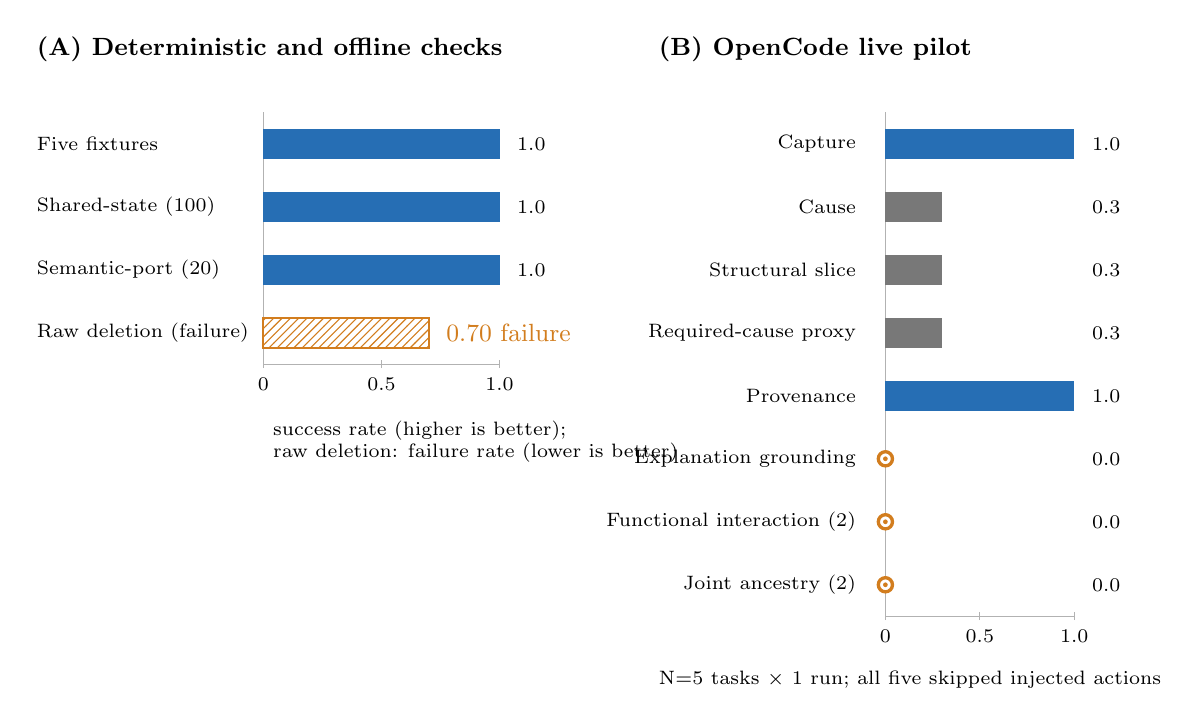
\begin{tikzpicture}[x=1cm,y=1cm,font=\scriptsize]
% Panel A: deterministic and offline checks
\begin{scope}
\node[anchor=west,font=\small\bfseries] at (0,8.2) {(A) Deterministic and offline checks};
\node[anchor=west] at (0,7.0) {Five fixtures};
\node[anchor=west] at (0,6.2) {Shared-state (100)};
\node[anchor=west] at (0,5.4) {Semantic-port (20)};
\node[anchor=west] at (0,4.6) {Raw deletion (failure)};
\draw[gray!60] (3.0,4.2)--(3.0,7.4);
\draw[gray!60] (3.0,4.2)--(6.0,4.2);
\fill[barblue] (3.0,6.81) rectangle (6.0,7.19);
\node[anchor=west] at (6.1,7.0) {1.0};
\fill[barblue] (3.0,6.01) rectangle (6.0,6.39);
\node[anchor=west] at (6.1,6.2) {1.0};
\fill[barblue] (3.0,5.21) rectangle (6.0,5.59);
\node[anchor=west] at (6.1,5.4) {1.0};
\draw[pattern=north east lines, pattern color=barorange, draw=barorange, thick] (3.0,4.41) rectangle (5.1,4.79);
\node[anchor=west, font=\small, text=barorange] at (5.2,4.6) {0.70 failure};
\draw[gray!60] (3.0,4.15)--(3.0,4.25);
\draw[gray!60] (4.5,4.15)--(4.5,4.25);
\draw[gray!60] (6.0,4.15)--(6.0,4.25);
\node at (3.0,3.95) {0};
\node at (4.5,3.95) {0.5};
\node at (6.0,3.95) {1.0};
\node[anchor=north west, font=\scriptsize, align=left] at (3.0,3.6) {success rate (higher is better);\\raw deletion: failure rate (lower is better)};
\end{scope}
% Panel B: OpenCode live pilot
\begin{scope}[shift={(7.9,0)}]
\node[anchor=west,font=\small\bfseries] at (0,8.2) {(B) OpenCode live pilot};
\node[anchor=east] at (2.75,7.0) {Capture};
\node[anchor=east] at (2.75,6.2) {Cause};
\node[anchor=east] at (2.75,5.4) {Structural slice};
\node[anchor=east] at (2.75,4.6) {Required-cause proxy};
\node[anchor=east] at (2.75,3.8) {Provenance};
\node[anchor=east] at (2.75,3.0) {Explanation grounding};
\node[anchor=east] at (2.75,2.2) {Functional interaction (2)};
\node[anchor=east] at (2.75,1.4) {Joint ancestry (2)};
\draw[gray!60] (3.0,1.0)--(3.0,7.4);
\draw[gray!60] (3.0,1.0)--(5.4,1.0);
\fill[barblue] (3.0,6.81) rectangle (5.4,7.19);
\node[anchor=west] at (5.5,7.0) {1.0};
\fill[bargray] (3.0,6.01) rectangle (3.72,6.39);
\node[anchor=west] at (5.5,6.2) {0.3};
\fill[bargray] (3.0,5.21) rectangle (3.72,5.59);
\node[anchor=west] at (5.5,5.4) {0.3};
\fill[bargray] (3.0,4.41) rectangle (3.72,4.79);
\node[anchor=west] at (5.5,4.6) {0.3};
\fill[barblue] (3.0,3.61) rectangle (5.4,3.99);
\node[anchor=west] at (5.5,3.8) {1.0};
\draw[barorange, very thick, fill=white] (3.0,3.0) circle (0.09);
  \fill[barorange] (3.0,3.0) circle (0.03);
\node[anchor=west] at (5.5,3.0) {0.0};
\draw[barorange, very thick, fill=white] (3.0,2.2) circle (0.09);
  \fill[barorange] (3.0,2.2) circle (0.03);
\node[anchor=west] at (5.5,2.2) {0.0};
\draw[barorange, very thick, fill=white] (3.0,1.4) circle (0.09);
  \fill[barorange] (3.0,1.4) circle (0.03);
\node[anchor=west] at (5.5,1.4) {0.0};
\draw[gray!60] (3.0,0.95)--(3.0,1.05);
\draw[gray!60] (4.2,0.95)--(4.2,1.05);
\draw[gray!60] (5.4,0.95)--(5.4,1.05);
\node at (3.0,0.75) {0};
\node at (4.2,0.75) {0.5};
\node at (5.4,0.75) {1.0};
\node[anchor=west] at (0,0.2) {N=5 tasks $\times$ 1 run; all five skipped injected actions};
\end{scope}
\end{tikzpicture}
\caption{Committed evaluation values. Panel A shows deterministic and offline checks; the final hatched bar is a raw-deletion failure rate (lower is better), not a success rate. Panel B shows the OpenCode pilot, with five tasks and one run each; all five runs skipped the injected actions. Capture is minimum expected event-class coverage, not precision or recall. Zero values in Panel B are open circles at the axis. No new measurements are added.}
\label{fig:bench}
\end{figure}

\noindent\textbf{Reading Figure~\ref{fig:bench}.} Panel A reports controlled deterministic and offline checks. The three 1.0 bars are success rates for the fixtures, shared-state recovery, and semantic-port replacement; they show that these controlled tests pass, not that the method is accurate in the field. The orange bar is not a success rate. It is the 70\% failure rate of raw text deletion (lower is better), a contrast condition: deleting a value emptied a required field, so parsing succeeded but schema validation failed and the decision was not evaluated, whereas semantic-port replacement kept the field shape and passed 20 of 20 cases. The bar therefore measures a schema failure, not a wrong decision.

\vspace{1em}

Panel B is smaller and weaker. Capture and provenance reach 1.0, but cause, structural slice, and required-cause preservation are 0.3, and explanation grounding, functional interaction, and joint ancestry are 0.0. Explanation grounding requires summary-level citations of recorded event IDs; package-level evidence alone does not pass. The interaction and joint-ancestry values are joint-branch ancestry detection, not causal interaction, and are measured on only two runs; the artifact marks true causal interaction as unsupported. 

\vspace{1em}

The pilot has five tasks with one run each, and all five runs skipped the injected actions, so it did not exercise the intended failure structure. The figure therefore shows a project that is instrumented and passes its deterministic tests; it does not demonstrate live diagnostic value, and it is not evidence that the project performed well or badly on real incidents.

\vspace{1em}

\noindent\textbf{What can be improved.} The next evaluation should use independent, held-out tasks with failures that actually occur, report the number of measurable runs for every metric, and require summary-level event-ID citations. Functional interaction should be tested only where a decision contract exists, with larger N, repeated runs, and concurrent-writer tests. A scored baseline would make the live panel informative. Until then, the figure is a progress report, not a claim of field performance.

\section{Limitations and Future Work}\label{sec:limits}
\subsection{Assumptions and threats to validity}
The replay analysis rests on five assumptions, each of which can fail:
\begin{itemize}
\item \textbf{Recorded graph completeness.} The analysis assumes that all relevant events and parent links were recorded. Missing instrumentation, dropped callbacks, or adapter order inference can omit a true dependency; the graph is not a complete causal model.
\item \textbf{No hidden confounders.} Replay assumes that the recorded ports and context contain the inputs that matter. Unrecorded external state can change the decision.
\item \textbf{Stable decision function.} Replay assumes the same deterministic decision code and evaluator between recording and replay. Code drift, a different policy version, or a changed evaluator invalidates the result.
\item \textbf{Ports are the only relevant inputs.} A contract must include every input that can change the decision. Missing ports produce incomplete sensitivity results.
\item \textbf{LLM nondeterminism and concurrent writers are untested.} The implemented replay is deterministic and makes no model calls; it does not repeat stochastic model decisions or estimate model uncertainty. The shared-state test has no concurrent writers or contention.
\end{itemize}
The fixture ground truth is co-authored with the fixtures, and the live pilot has one run per task, so internal and external validity are both limited.

\subsection{Limitations}
\begin{itemize}
\item \textbf{Declared dependence is not proof.} A slice shows structural ancestry, not that each event changed the outcome. Some adapter edges are order-inferred rather than declared.
\item \textbf{Model internals.} Once a value passes through a language model the link is coarse; the system cannot look inside the model.
\item \textbf{Replay limits.} Replay calls a registered evaluator and cannot inspect it. Evaluators must be pure; the side-effect guard is metadata- and value-based and is not a sandbox. Impure evaluators can repeat external actions.
\item \textbf{Deterministic replay only.} The implementation does not repeat language-model calls or sample stochastic decisions. Its duplicate evaluations are deterministic copies, not stochastic trials, and we draw no model-uncertainty conclusion from them.
\item \textbf{Per-agent reconstruction.} State reconstruction is per agent; snapshots are optional and are not used by the default analysis path. Global cross-agent state is not reconstructed.
\item \textbf{Scale and live traces.} Exact subset enumeration supports up to four decision ports. Functional-interaction claims from live traces are not supported; the pilot reports joint-ancestry and functional-interaction scores, both 0.0.
\item \textbf{Explanation grounding.} The structural-slice note is systematic, but there is no general verifier that every sentence is supported by recorded evidence. The live pilot's explanation grounding score is 0.0.
\item \textbf{Untested integrations.} Apart from LangGraph and OpenCode, the integrations in Table~\ref{tab:tools} are proposed.
\end{itemize}

\subsection{Future work}
The next steps are independent, held-out labels; repeated live runs with variance reporting; stochastic replay that records model samples rather than assuming determinism; concurrent-writer and race tests; an edge-type field that distinguishes declared from order-inferred links; a sandbox for pure evaluators; snapshot-backed and cross-agent reconstruction; and evaluated integrations beyond the two adapters.

\section{Related Work}\label{sec:related}
The system applies established ideas in a new setting. Program slicing~\cite{weiser1981} reduces a program to the statements that affect a value; the structural slice does the same for a recorded agent run. Delta debugging~\cite{zeller2002} shrinks a failing input to a smaller one. Logical clocks~\cite{lamport1978} order events in distributed systems. Shapley values~\cite{shapley1953} and functional-interaction indices~\cite{grabisch1999} come from cooperative game theory. Our local replay is inspired by the intervention view of causality~\cite{pearl2009}, but it does not identify causal effects.

Distributed tracing systems such as Dapper~\cite{dapper2010} and the OpenTelemetry tracing model~\cite{opentelemetry2025} record spans and parent--child context across services. They provide the trace substrate; they do not by themselves encode a data-dependency edge or a decision contract. Work on database provenance~\cite{cheney2009} distinguishes why, how, and where provenance; our exact and coarse grades are a deliberately small engineering approximation of that space, not a full provenance model.

Halpern and Pearl~\cite{halpern2005} define actual causes with structural counterfactuals. Our replay is weaker: it intervenes on recorded ports of a registered evaluator and observes a functional change, without modeling hidden confounders or estimating a causal effect. Recent work on failure attribution in multi-agent systems includes the Who\&When benchmark and methods~\cite{zhang2025}, the MAST failure taxonomy~\cite{cemri2025}, and the TRAIL trace benchmark~\cite{trail2025}. These localize failing agents or steps from annotated traces; our question is complementary and narrower: whether recorded inputs, alone or jointly, change a merge decision in replay.

The defensible novelty is therefore narrow: a contract-based method for testing whether recorded inputs, alone or jointly, change a merge decision, with explicit provenance caveats and an implementation that separates structural ancestry from functional influence.

\section{Conclusion}
Agent-Causality records what agents did as a dependency graph with parent links, uses structural slices and exact/coarse provenance to show what a failure is connected to, and tests deterministic functional influence on registered merge decisions. Its main contribution is separating three things that logs blur together: what happened, what a failure is structurally connected to, and what changed a registered decision in replay. It does not establish actual causation, and it is explicit about order-inferred edges, deterministic replay, per-agent reconstruction, and the limits of its evaluation. Alone, it helps developers inspect and audit multi-agent runs; combined with approval tools, test pipelines, security gateways and incident tools, it could turn the graph into automated checks and shared evidence, but those combinations are proposed rather than evaluated. Independent evaluation on live systems, stochastic decisions, concurrent writers, and tested integrations are the main next steps.

\begin{thebibliography}{15}\small
\bibitem{lamport1978} L.~Lamport. Time, clocks, and the ordering of events in a distributed system. \emph{Communications of the ACM}, 21(7):558--565, 1978.
\bibitem{weiser1981} M.~Weiser. Program slicing. In \emph{Proc. 5th International Conference on Software Engineering}, pp.~439--449, 1981.
\bibitem{shapley1953} L.~S. Shapley. A value for $n$-person games. In H.~W. Kuhn and A.~W. Tucker, editors, \emph{Contributions to the Theory of Games II}, pp.~307--317. Princeton University Press, 1953.
\bibitem{zeller2002} A.~Zeller and R.~Hildebrandt. Simplifying and isolating failure-inducing input. \emph{IEEE Transactions on Software Engineering}, 28(2):183--200, 2002.
\bibitem{grabisch1999} M.~Grabisch and M.~Roubens. An axiomatic approach to the concept of interaction among players in cooperative games. \emph{International Journal of Game Theory}, 28:547--565, 1999.
\bibitem{pearl2009} J.~Pearl. \emph{Causality: Models, Reasoning, and Inference}, 2nd ed. Cambridge University Press, 2009.
\bibitem{fortune2025} B.~Nolan. An AI-powered coding tool wiped out a software company's database, then apologized for a ``catastrophic failure on my part''. \emph{Fortune}, July 23, 2025. \url{https://fortune.com/2025/07/23/ai-coding-tool-replit-wiped-database-called-it-a-catastrophic-failure/}. Accessed 22 October 2026.
\bibitem{ars2025} B.~Edwards. Two major AI coding tools wiped out user data after making cascading mistakes. \emph{Ars Technica}, July 24, 2025. \url{https://arstechnica.com/information-technology/2025/07/ai-coding-assistants-chase-phantoms-destroy-real-user-data/}. Accessed 22 October 2026.
\bibitem{dapper2010} B.~H. Sigelman, L.~A. Barroso, M.~Burrows, P.~Stephenson, M.~Plakal, D.~Beaver, S.~Jaspan, and C.~Shanbhag. Dapper, a large-scale distributed systems tracing infrastructure. Technical Report dapper-2010-1, Google, April 2010.
\bibitem{opentelemetry2025} OpenTelemetry Authors. OpenTelemetry documentation: traces. \url{https://opentelemetry.io/docs/concepts/signals/traces/}. Accessed 22 October 2026.
\bibitem{cheney2009} J.~Cheney, L.~Chiticariu, and W.-C. Tan. Provenance in databases: Why, how, and where. \emph{Foundations and Trends in Databases}, 1(4):379--474, 2009. DOI: 10.1561/1900000006.
\bibitem{halpern2005} J.~Y. Halpern and J.~Pearl. Causes and explanations: A structural-model approach. Part I: Causes. \emph{British Journal for the Philosophy of Science}, 56(4):843--887, 2005. DOI: 10.1093/bjps/axi148.
\bibitem{zhang2025} S.~Zhang, M.~Yin, J.~Zhang, J.~Liu, Z.~Han, J.~Zhang, B.~Li, C.~Wang, H.~Wang, Y.~Chen, and Q.~Wu. Which agent causes task failures and when? On automated failure attribution of LLM multi-agent systems. In \emph{Proc. 42nd International Conference on Machine Learning (ICML)}, 2025. arXiv:2505.00212.
\bibitem{cemri2025} M.~Cemri, M.~Z. Pan, S.~Yang, L.~A. Agrawal, B.~Chopra, R.~Tiwari, K.~Keutzer, A.~Parameswaran, D.~Klein, et al. Why do multi-agent LLM systems fail? In \emph{NeurIPS 2025 Datasets and Benchmarks Track}, 2025. arXiv:2503.13657.
\bibitem{trail2025} D.~Deshpande, V.~Gangal, H.~Mehta, J.~Krishnan, A.~Kannappan, and R.~Qian. TRAIL: Trace reasoning and agentic issue localization. arXiv:2505.08638, 2025.
\end{thebibliography}
\end{document}
